\chapter{针对形变的理论建模}

\section{使用数据}
使用上一章得到的平均形变速率作为建模的输入数据,
对于该区域中部的明显形变采用mogi模型建模。

\section{mogi模型}
mogi模型为最常用的点源模型。
它的基本假设为:
\begin{enumerate}
    \item 介质为各项同性线性弹性介质,可以用剪切模量$\mu$和泊松比$\nu$完全表征介质的特性。
    \item 研究空间为半空间。
    \item 扰动源为点源,即源的尺度远小于模型的尺度:$\alpha \ll d$。
\end{enumerate}

由以上基本假设可以得知,mogi模型的参数分为两个部分:
\begin{enumerate}
    \item 扰动源的参数:扰动源的位置$X,Y,Z$,以及表征扰动大小的体应变$DV$。
    \item 介质的参数:剪切模量$\mu$和泊松比$\nu$。
\end{enumerate}
其中地球介质的参数波动不大,一般设成已知量,对反演的结果影响不大。
主要的反演参数为扰动源的四个参数。

\section{建模软件}
本研究使用的建模软件为GBIS,关于反演算法和软件已经在第\ref{ch:pm}章中说明。

\section{反演过程和结果}
为了节省运算时间,首先对数据进行quadtree重采样,
采样前后的对比如图\ref{fig:unsample}和\ref{fig:subsample}所示。
\begin{figure}[htp]
    \centering
    \begin{minipage}{0.9\textwidth}
        \centering
        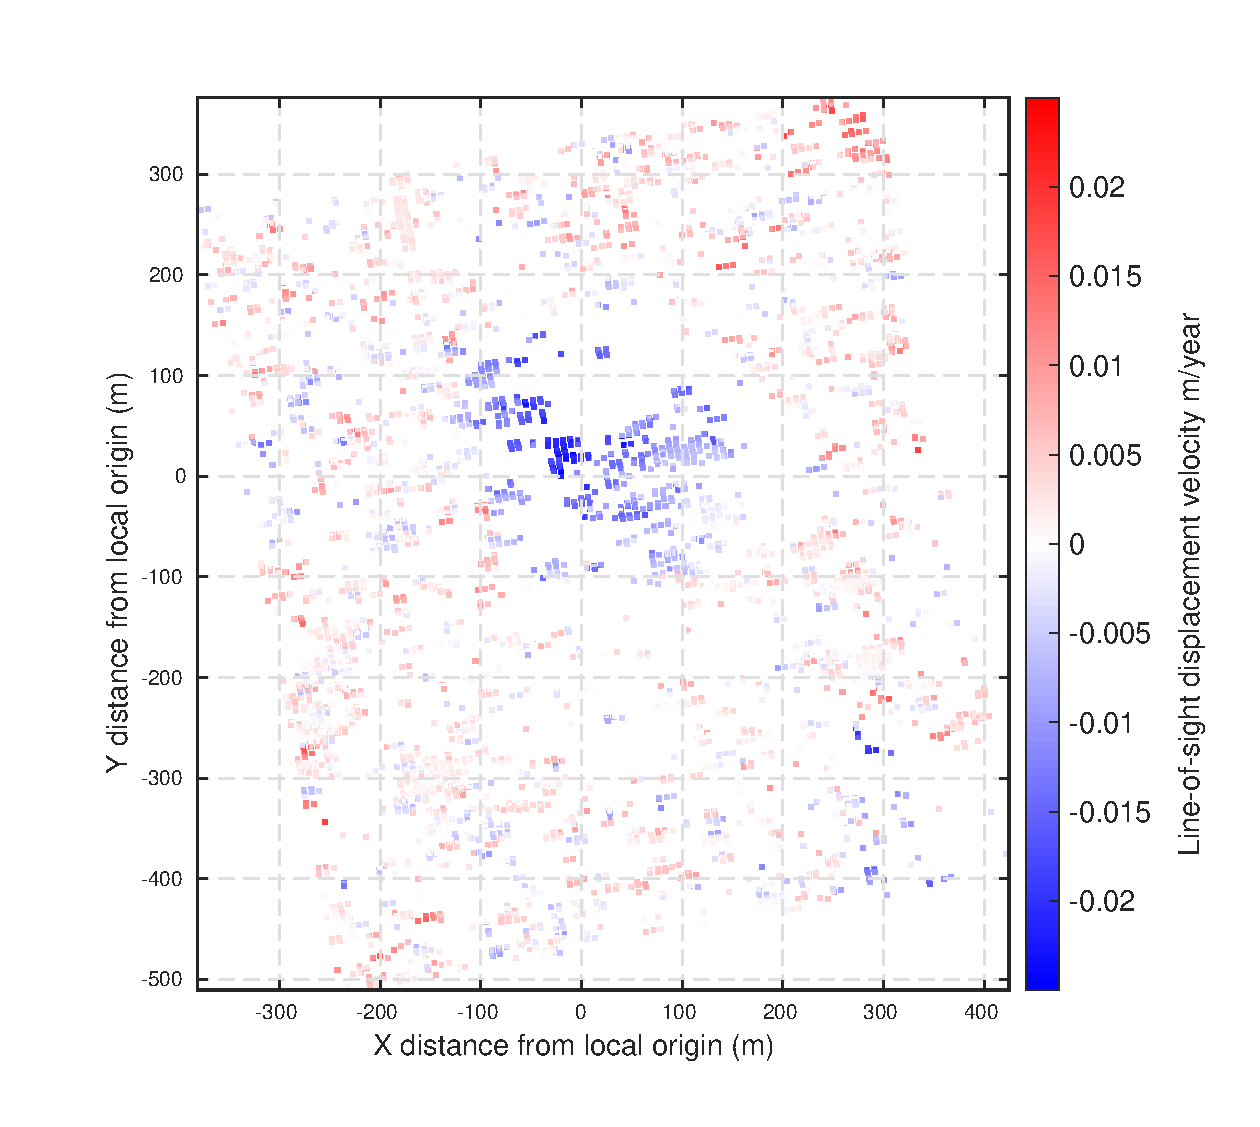
\includegraphics[width=0.8\textwidth]{unwrapped.eps}
        \caption{原始形变图}
        \label{fig:unsample}
    \end{minipage}
    \qquad
    \begin{minipage}{0.9\textwidth}
        \centering
        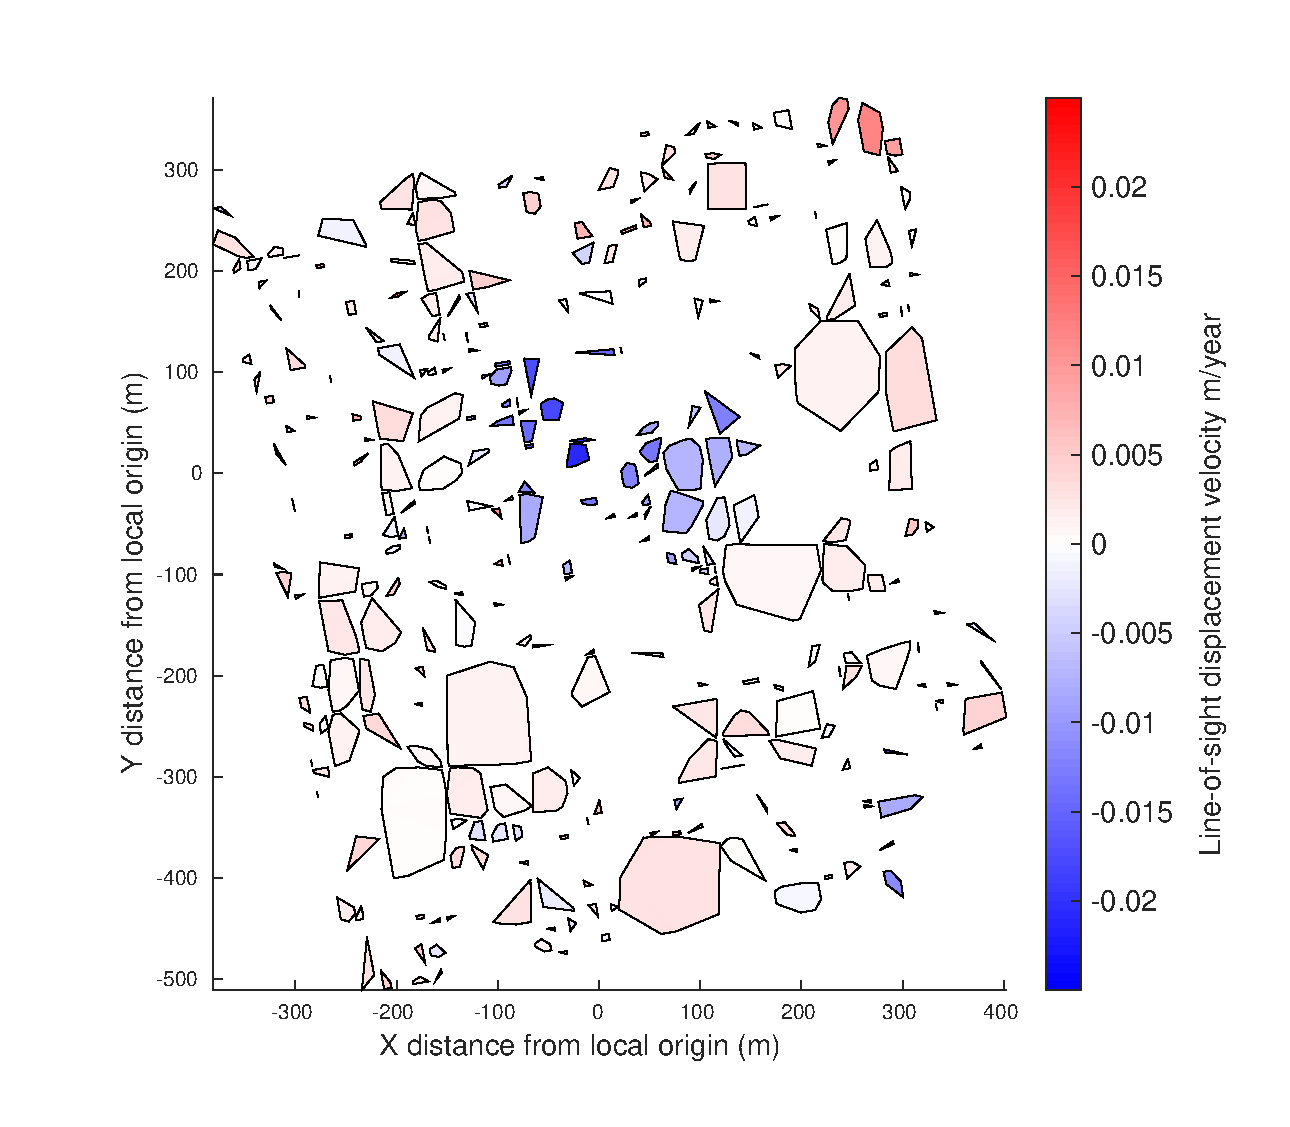
\includegraphics[width=0.8\textwidth]{subsampled.eps}
        \caption{quadtree采样后的形变图}
        \label{fig:subsample}
    \end{minipage}
%    \caption{aaa}
%    \label{zhong}
\end{figure}
然后开始反演。反演的结果见表\ref{tab:modelpar}。
\begin{table}[htb]
    \centering\small
    \caption{模型参数}
    \label{tab:modelpar}
    \begin{tabular}{@{}cccccc@{}}
    \toprule
    参数       & 最优值 & 平均值 & 中位值 & 2.5\% & 97.5\% \\ 
    \midrule
    mogi X    & -14.20 & -13.19 &-12.59 & -50.51 & 10.94 \\
    mogi Y     & 45.89 & 46.84 & 46.34 & 18.01 & 78.61\\
    mogi depth & 103.57 & 114.46 & 105.80 & 85.44 & 238.95\\
    mogi DV   & -1121.93 & -1240.33 & -1111.70 & -3228.15 & -713.27\\
    InSAR 常数 & 0.00 & 0.00 & 0.00 & -0.00 & 0.01\\
    \bottomrule
    \end{tabular}
\end{table}
参数的后验概率见图\ref{fig:pdf}。
从该图中可以看出,X,Y的后验概率分布比较散,这两个参数的收敛性较差。
\begin{figure}[htb]
    \centering
    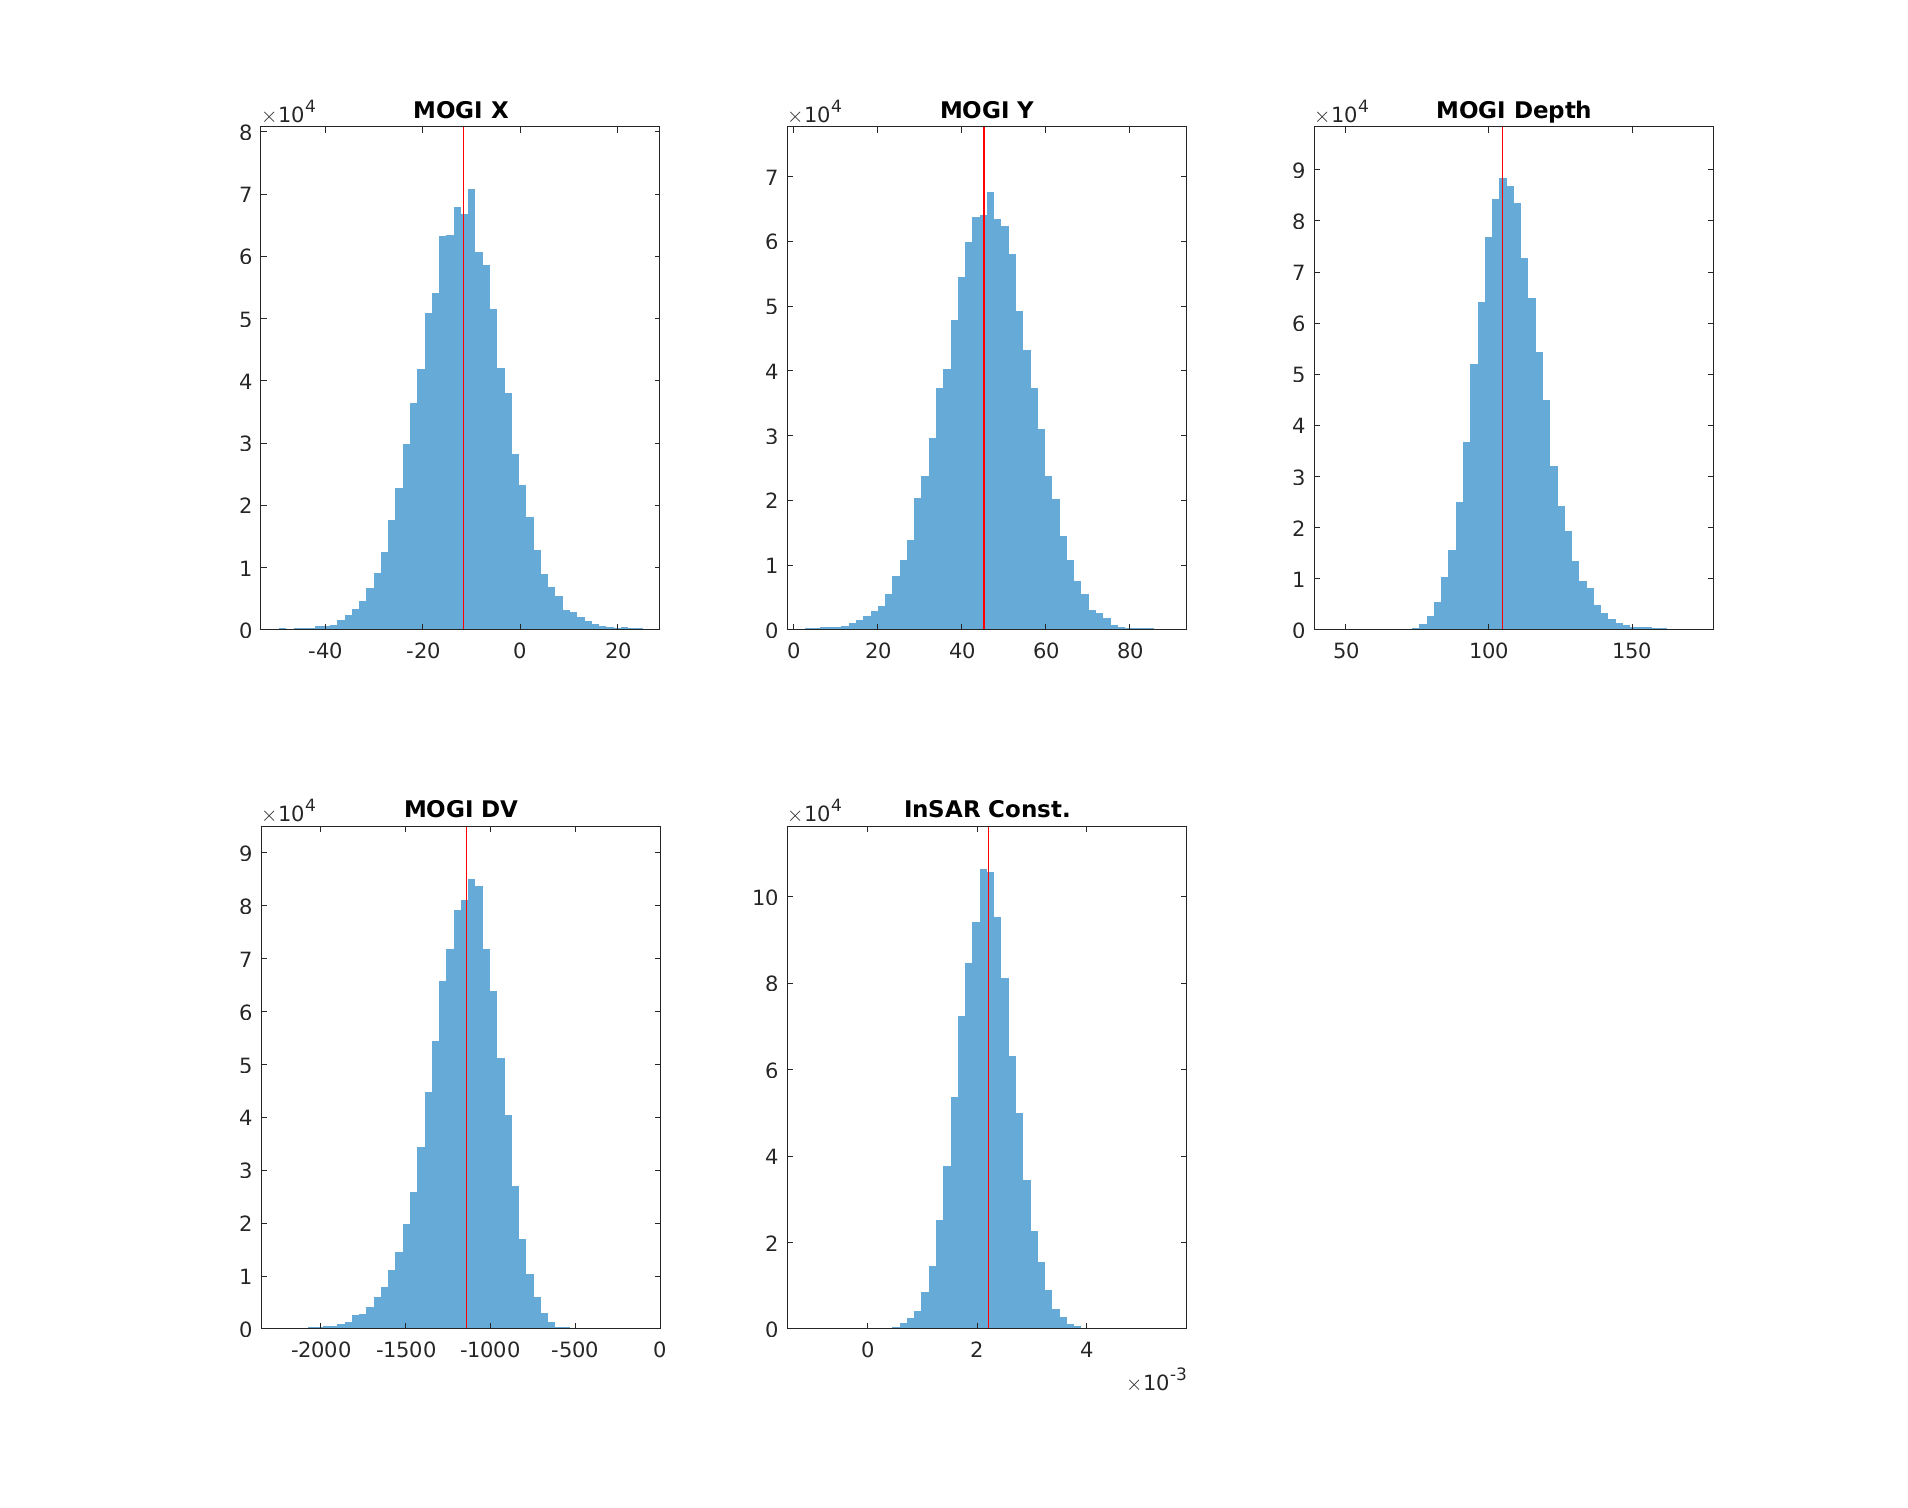
\includegraphics[width=1.0\textwidth]{PDFs.eps}
    \caption{反演参数的后验概率分布}
    \label{fig:pdf}
\end{figure}
原始形变数据,反演参数理论行便和二者的差见图\ref{fig:residual}。
\begin{figure}[htb]
    \centering
    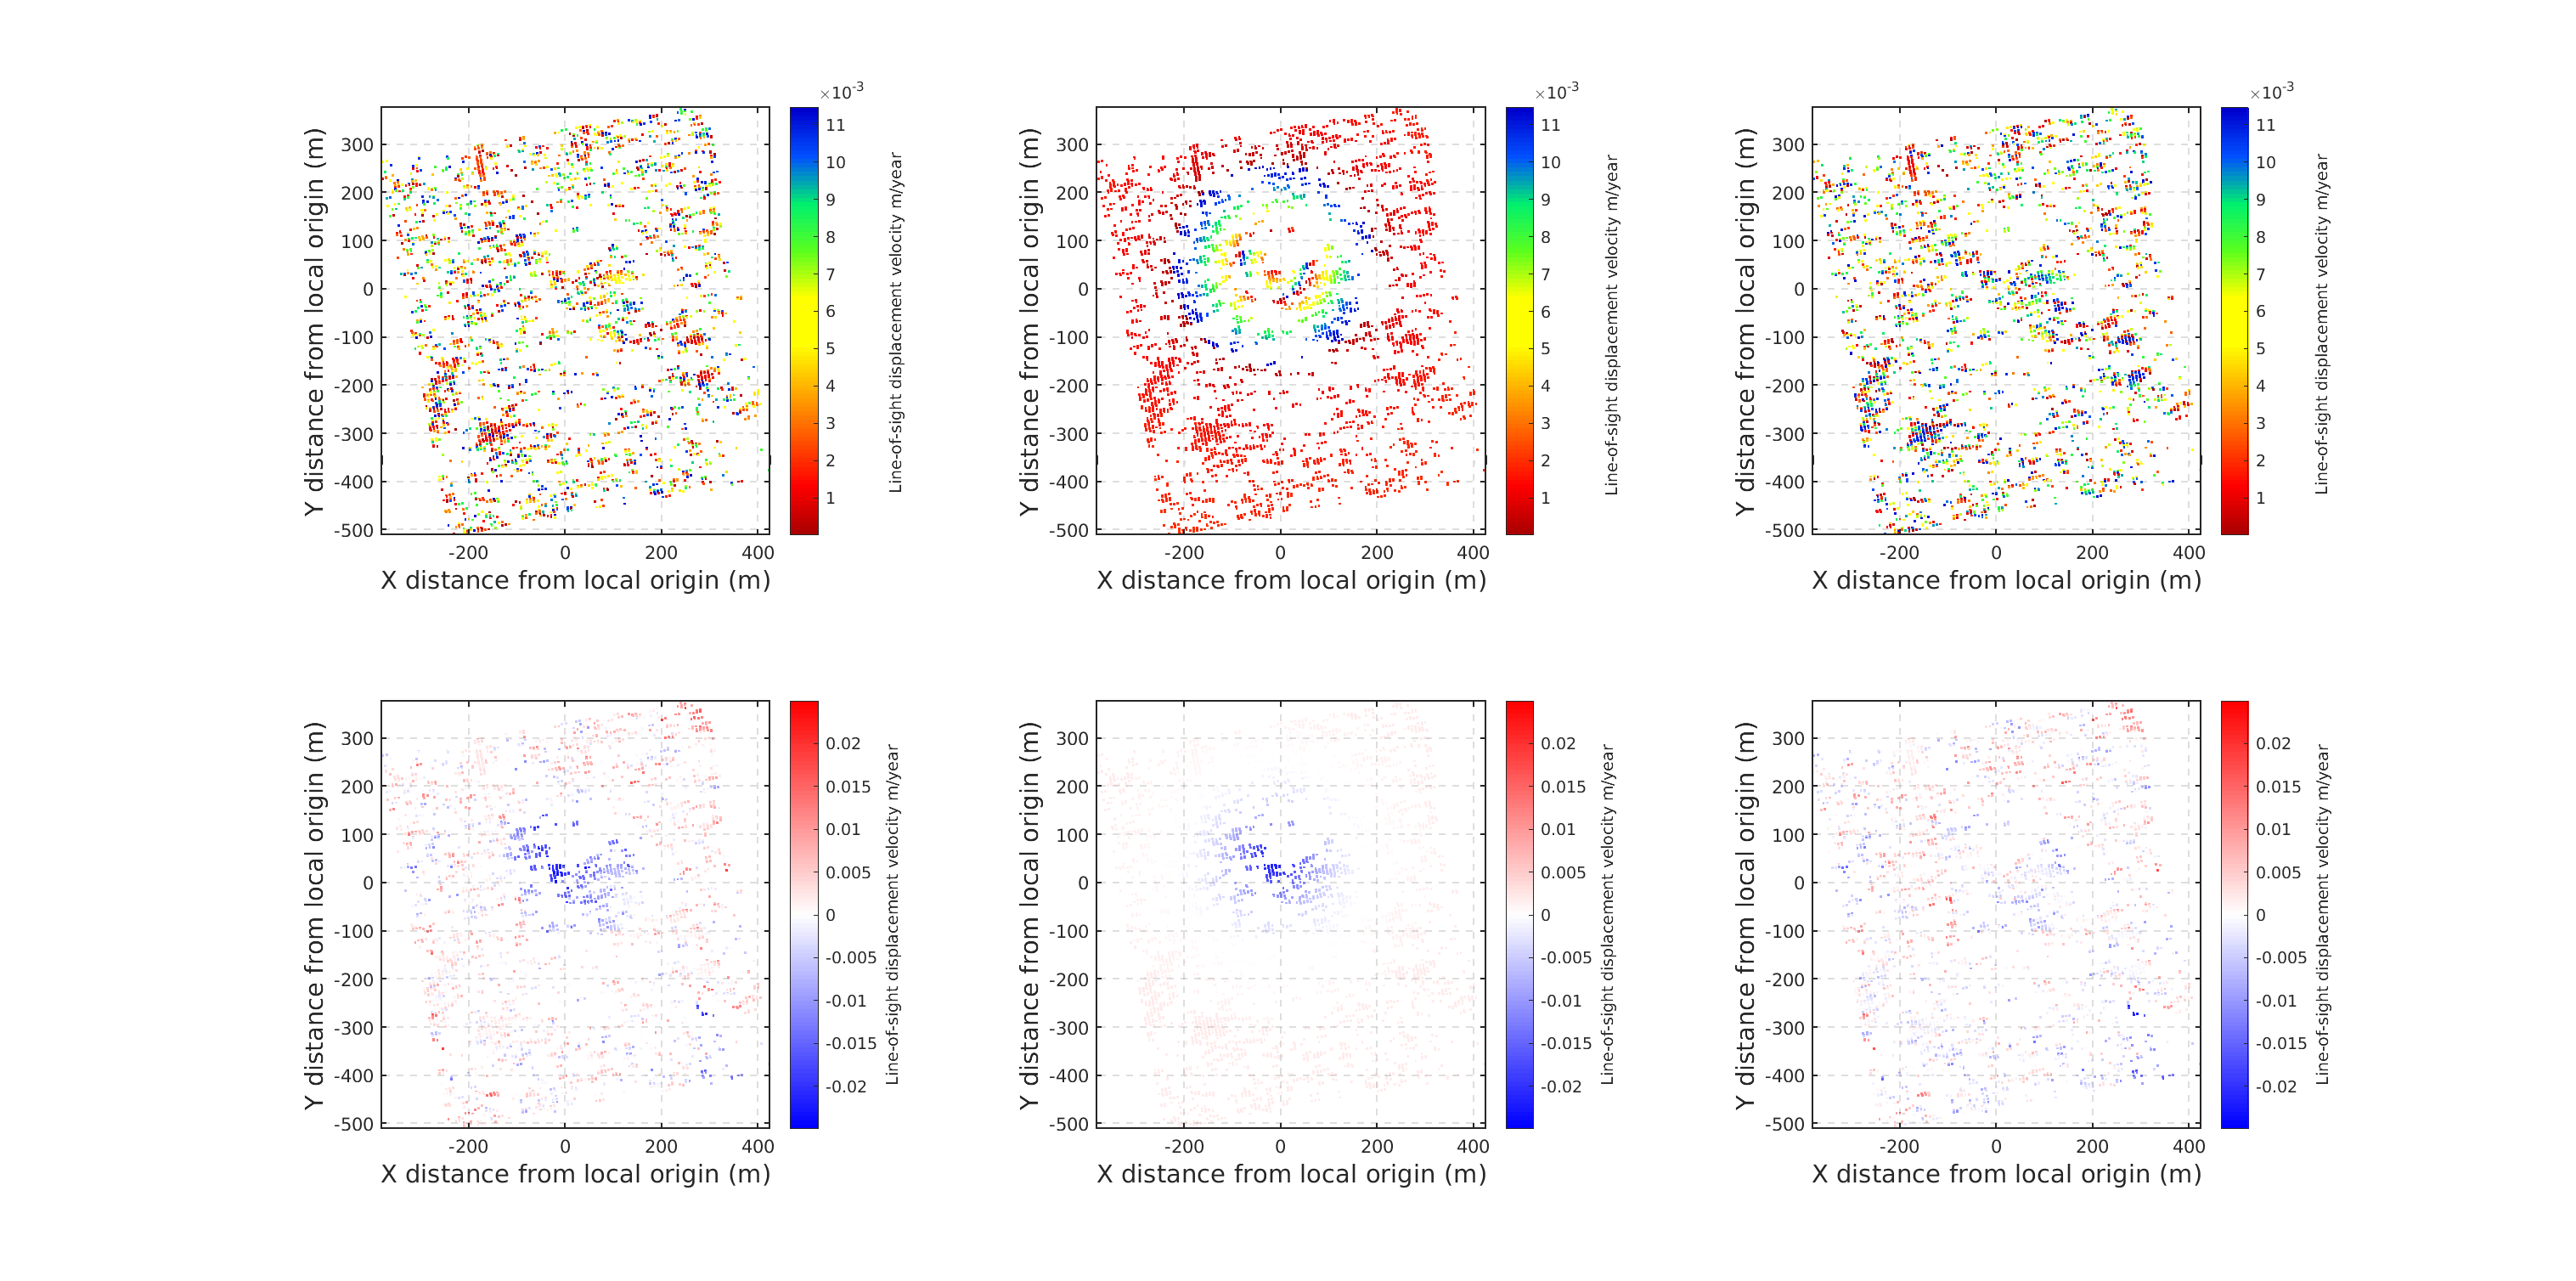
\includegraphics[width=1.0\textwidth]{residual.eps}
    \caption{原始形变数据,反演参数理论形变以及二者的差}
    \note{注:六副图中,上面三副为未解缠的数据,下面三副为解缠之后的数据;
    左边的图为原始形变的数据,中间的图为模型理论推导的形变数据,右边为原始数据减去理论数据的剩余数据。}
    \label{fig:residual}
\end{figure}
从图\ref{fig:residual}来看,反演比较成功,模型反推的结果和InSAR观测的结果吻合得比较好。
但从图中可以看出,InSAR的结果仍有很多不吻合的地方。
一方面,可能是数据处理的原因,本研究分析的区域较小,大概在1平方公里左右,
所得到的PS点也不够密集,不一定能比较全面地覆盖当地的所有形变特征。
另一方面,也有可能是模型较为粗糙的原因,mogi模型是比较简单的模型,
可能实际导致形变的扰动源比较复杂。
从图\ref{fig:residual}中的剩余形变图可以看出,该区域的下半部分有不太明显的下沉,上半部分有一定的上升,
这部分的形变没有被mogi模型解释,如果采用更精确的模型,可能会有更好的反演效果。